\documentclass[UTF8]{ctexbook}
\usepackage{tikz}
\usetikzlibrary{arrows.meta}
\usepackage[siunitx]{circuitikz}
\usepackage{graphicx}
\usepackage{wrapfig}
\usepackage{amsmath,amssymb}
\usepackage{xcolor}
\usepackage{geometry}
\geometry{a4paper,margin=2.5cm}
\sisetup{inter-unit-product = \ensuremath{{}\cdot{}}}
\definecolor{elecblue}{RGB}{0,155,220} % 电路图用的蓝色

\begin{document}
\chapter*{第一章 Circuit Variables}

\section{国际单位制与前缀}
\noindent
\begin{minipage}[t]{0.48\textwidth}
\subsection{SI 基本量与基本单位}
\begin{itemize}
  \item 长度:meter(米),符号 m
  \item 质量:kilogram(千克),符号 kg
  \item 时间:second(秒),符号 s
  \item 电流:ampere(安培),符号 A
  
$1~\si{\ampere} = 1~\si{\coulomb\per\second}$
  \item 热力学温度:kelvin(开尔文),符号 K
  \item 物质的量:mole(摩尔),符号 mol
  \item 发光强度:candela(坎德拉),符号 cd
\end{itemize}
\subsection{十进制前缀}
\begin{center}
\begin{tabular}{ll}
nano, n: $10^{-9}$ & giga, G: $10^{9}$\\
micro, $\mu$: $10^{-6}$ & mega, M: $10^{6}$\\
milli, m: $10^{-3}$ & kilo, k: $10^{3}$
\end{tabular}
\end{center}
\end{minipage}%
\hfill
\begin{minipage}[t]{0.48\textwidth}
\subsection*{常见导出单位}
\begin{itemize}
  \item 频率:hertz(赫兹),符号Hz

\noindent$1~\text{Hz}=1~\si{\per\second}$。
  \item 力:newton(牛顿),符号N

\noindent$1~\si{\newton} = 1~\si{\kilogram\metre\per\second\squared}$。
  \item 能量:joule(焦耳),符号J

\noindent$1~\text{J}=1~\si{\newton\meter}$。
  \item 功率:watt(瓦特),符号W

\noindent$1~\text{W}=1~\si{\joule\per\second}$。
  \item 电荷:coulomb(库伦),符号C

\noindent$1~\text{C}=1~\si{\ampere\second}$。
  \item 电压:volt(伏特),符号V

\noindent$1~\text{V}=1~\si{\joule\per\coulomb}$。
\end{itemize}
\end{minipage}
\section{电压与电流}

\subsection{电荷与电子电荷}
\begin{itemize}
  \item 电荷是所有电学现象的基础,具有\textbf{正负两种极性}。

\noindent 单位是库伦:$\si{\coulomb}$
\[
1~\si{\coulomb} = 6.24~\si{\times10}^{18}{e}.
\]
\noindent 最小单位为电子电荷
  \[
    q_e = 1.6022\times 10^{-19}\ \text{C}.
  \]
\end{itemize}

\subsection{电压(电势差)的定义}
\noindent 电荷从一端移动到另一端需要消耗能量,每单位电荷所需的能量称为电压:
\begin{equation}
  v = \frac{\mathrm{d}w}{\mathrm{d}q}\quad [\text{V}],
\end{equation}
\noindent 其中 $w$ 为能量(J),$q$ 为电荷(C)。

\noindent 单位是伏特:
\[
1~\si{\volt} = 1~\si{\joule\per\coulomb}.
\]
\subsection{能量与电压的关系}
\noindent
 \paragraph*{能量}:电压对电荷量积分
  \[
    w(t) = \int_{q_{t_0}}^{q_t} \si{\volt}\mathrm{d}q
  \]
\subsection{电流的定义}

\noindent 单位时间内通过某一截面的电荷量称为电流:
\begin{equation}
  i = \frac{\mathrm{d}q}{\mathrm{d}t}\quad [\text{A}],
\end{equation}

\noindent 其中 $q$ 为通过截面的净电荷,$t$ 为时间。

正电流按约定对应\textbf{正电荷}沿\emph{参考方向}的流动。

\noindent 单位是安培:
\[
  1~\si{\ampere} = 1~\si{\coulomb\per\second}.
\]

\paragraph{\noindent (a)直流电流(direct current):}是不随时间变化的恒定电流

\paragraph{\noindent (b)交流电流(alternating current):}是随时间按正弦规律变化的电流

\begin{figure}[htbp]
  \centering

  %========= 左边:上方那幅直流电流图 =========
  \begin{minipage}[b]{0.45\textwidth}
    \centering
    \begin{tikzpicture}[>=stealth, scale=1.2]
      % 这里放你“上面那幅图”的代码
      \draw[->] (-1,0) -- (4,0) node[below] {$t$};
      \draw[->] (0,-0.5) -- (0,3) node[left] {$I$};
      \node[below left] at (0,0) {$0$};
      \draw[thick,red] (-0.8,2) -- (3,2);
      \node[left] at (-0.9,2) {$i_s$};
    \end{tikzpicture}
    \\(a)
  \end{minipage}
  \hfill
  %========= 右边:下方那幅交流电流图 =========
  \begin{minipage}[b]{0.45\textwidth}
    \centering
    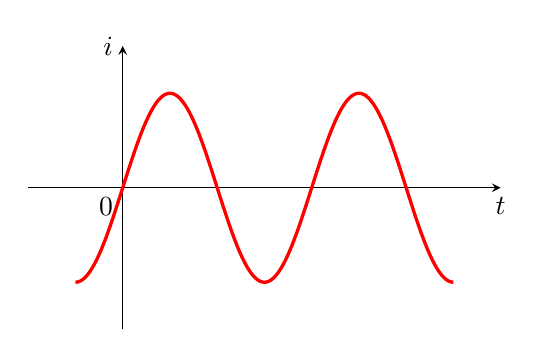
\begin{tikzpicture}[>=stealth, scale=1.2]
      % 这里放你“下面那幅图”的代码
      \draw[->] (-1,0) -- (4,0) node[below] {$t$};
      \draw[->] (0,-1.5) -- (0,1.5) node[left] {$i$};
      \node[below left] at (0,0) {$0$};

      \draw[very thick, red, domain=-0.5:3.5, samples=200, smooth]
        plot (\x,{sin(180*\x)});
    \end{tikzpicture}
    \\(b)
  \end{minipage}

\end{figure}

\subsection{电荷量与电流的关系}
\noindent 时刻$t_{0}$到$t$之间的电荷量:
\[
    Q = \int_{t_0}^{t} i\,\mathrm{d}t
\]

\section{理想基本电路元件与参考方向}
\subsection{理想基本电路元件的三个特征}
\noindent
\begin{minipage}[t]{0.9\textwidth}   % 左列:文字
\begin{enumerate}
  \item \textbf{只有两个端口}:仅通过这两个端口与外部电路连接。
  \item \textbf{可用 $v$、$i$ 的关系精确描述}:$v$–$i$ 关系是该元件的全部电气特性。
  \item \textbf{不可再分}:不能再用更简单的电路元件去建模它——它本身就是模型的“原子”。
\end{enumerate}
\end{minipage}%

\hfill
\begin{minipage}[c]{0.2\textwidth}    % 右列:图形
  \centering
   \vspace{-9em}     
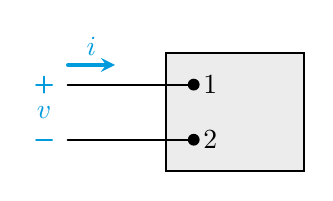
\begin{tikzpicture}[>=stealth, line cap=round, scale=0.5]

  % 右侧灰色方块(器件)
  \fill[gray!15] (2.5,-1.5) rectangle (6,1.5);
  \draw[thick]   (2.5,-1.5) rectangle (6,1.5);

  % 上、下导线
  \draw[thick] (0,0.7) -- (3.2,0.7);
  \draw[thick] (0,-0.7) -- (3.2,-0.7);

  % 器件左侧竖线和端点
  \draw[thick] (2.5,0.7) -- (2.5,-0.7);
  \fill (3.2,0.7) circle (0.15);
  \fill (3.2,-0.7) circle (0.15);

  % 端子编号 1、2
  \node[right] at (3.2,0.7) {$1$};
  \node[right] at (3.2,-0.7) {$2$};

  % 电压极性 + / - (蓝色)
  \draw[elecblue, thick] (-0.8,0.7) -- (-0.4,0.7); % 顶部横线
  \draw[elecblue, thick] (-0.6,0.5) -- (-0.6,0.9); % 竖线成 +
  \draw[elecblue, thick] (-0.8,-0.7) -- (-0.4,-0.7); % 底部横线成 -

  % 电压标注 v
  \node[elecblue] at (-0.6,0) {$v$};

  % 电流箭头 i(蓝色)
  \draw[elecblue, very thick, ->] (0,1.2) -- (1.2,1.2);
  \node[above, elecblue] at (0.6,1.2) {$i$};

\end{tikzpicture}
\end{minipage}

\subsection{电压极性与电流参考方向}
\noindent
\begin{minipage}[t]{0.6\textwidth}  % 左列:文字
\noindent 对任一双端口元件,都需要约定:
\begin{itemize}
  \item 电压的\textbf{参考极性}:用 “$+$” 和 “$-$” 标在两端子上。
  \item 电流的\textbf{参考方向}:用箭头指明正电流方向。
\end{itemize}
\noindent 数值的正负含义(以$v$从1到2为参考极性):
\begin{itemize}
  \item $v>0$:1 端比 2 端电势高(1→2 为电压“降”)。
  \item $v<0$:1 端比 2 端电势低(1→2 实际为电压“升”)。
  \item $i>0$:正电荷从 1 端流向 2 端。
  \item $i<0$:正电荷从 2 端流向 1 端。
\end{itemize}
\end{minipage}%

\hfill
\begin{minipage}[t]{0.38\textwidth}  % 右列:4 个小图
  \vspace{-16em}  
  \centering
  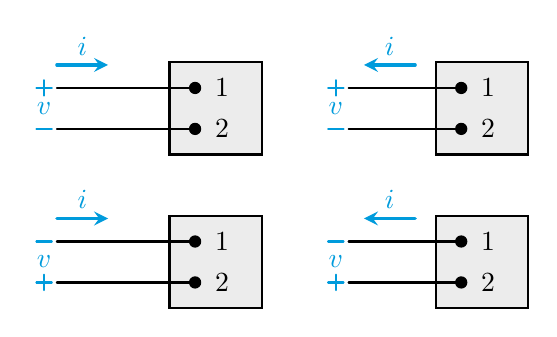
\begin{tikzpicture}[>=stealth, line cap=round, scale=0.65]

    % 一个小电路块的封装:参数为 (是否反极性, 是否反电流方向, 标号)
    % 这里直接展开写,方便你看和改

    % ---------- (a) p = vi ----------
    \begin{scope}[shift={(0,0)}]
      % 灰块和导线
      \fill[gray!15] (1,-0.9) rectangle (2.8,0.9);
      \draw[thick]   (1,-0.9) rectangle (2.8,0.9);
      \draw[thick] (-1.2,0.4) -- (1.5,0.4);
      \draw[thick] (-1.2,-0.4) -- (1.5,-0.4);
      \fill (1.5,0.4) circle (0.12);
      \fill (1.5,-0.4) circle (0.12);
      \node[right] at (1.7,0.4) {$1$};
      \node[right] at (1.7,-0.4) {$2$};

      % 电压极性 + / -
      \draw[elecblue, thick] (-1.6,0.4) -- (-1.3,0.4);
      \draw[elecblue, thick] (-1.45,0.25) -- (-1.45,0.55); % 竖线成 +
      \draw[elecblue, thick] (-1.6,-0.4) -- (-1.3,-0.4);  % -

      % v
      \node[elecblue] at (-1.45,0) {$v$};

      % 电流 i:从左到右
      \draw[elecblue, very thick, ->] (-1.2,0.85) -- (-0.2,0.85);
      \node[above, elecblue] at (-0.7,0.85) {$i$};

      % 标号
    \end{scope}

    % ---------- (b) p = -vi ----------
    \begin{scope}[shift={(4.5,0)}]
      \fill[gray!15] (1.7,-0.9) rectangle (3.5,0.9);
      \draw[thick]   (1.7,-0.9) rectangle (3.5,0.9);
      \draw[thick] (0,0.4) -- (2.2,0.4);
      \draw[thick] (0,-0.4) -- (2.2,-0.4);
      \fill (2.2,0.4) circle (0.12);
      \fill (2.2,-0.4) circle (0.12);
      \node[right] at (2.4,0.4) {$1$};
      \node[right] at (2.4,-0.4) {$2$};

      % 同样的极性 + / -
      \draw[elecblue, thick] (-0.4,0.4) -- (-0.1,0.4);
      \draw[elecblue, thick] (-0.25,0.25) -- (-0.25,0.55);
      \draw[elecblue, thick] (-0.4,-0.4) -- (-0.1,-0.4);
      \node[elecblue] at (-0.25,0) {$v$};

      % 电流 i:从右到左(反方向)
      \draw[elecblue, very thick, <-] (0.3,0.85) -- (1.3,0.85);
      \node[above, elecblue] at (0.8,0.85) {$i$};

    \end{scope}

    % ---------- (c) p = -vi ----------
    \begin{scope}[shift={(0,-3)}]
      \fill[gray!15] (1,-0.9) rectangle (2.8,0.9);
      \draw[thick]   (1,-0.9) rectangle (2.8,0.9);
      \draw[thick] (-1.2,0.4) -- (1.5,0.4);
      \draw[thick] (-1.2,-0.4) -- (1.5,-0.4);
      \fill (1.5,0.4) circle (0.12);
      \fill (1.5,-0.4) circle (0.12);
      \node[right] at (1.7,0.4) {$1$};
      \node[right] at (1.7,-0.4) {$2$};

      % 极性反过来:上端 -
      \draw[elecblue, thick] (-1.6,-0.4) -- (-1.3,-0.4); % 上下对调
      \draw[elecblue, thick] (-1.6,0.4) -- (-1.3,0.4);
      \draw[elecblue, thick] (-1.45,-0.55) -- (-1.45,-0.25); % + 在下端
      \node[elecblue] at (-1.45,0) {$v$};

      % 电流 i:从左到右
      \draw[elecblue, very thick, ->] (-1.2,0.85) -- (-0.2,0.85);
      \node[above, elecblue] at (-0.7,0.85) {$i$};

    \end{scope}

    % ---------- (d) p = vi ----------
    \begin{scope}[shift={(4.5,-3)}]
      \fill[gray!15] (1.7,-0.9) rectangle (3.5,0.9);
      \draw[thick]   (1.7,-0.9) rectangle (3.5,0.9);
      \draw[thick] (0,0.4) -- (2.2,0.4);
      \draw[thick] (0,-0.4) -- (2.2,-0.4);
      \fill (2.2,0.4) circle (0.12);
      \fill (2.2,-0.4) circle (0.12);
      \node[right] at (2.4,0.4) {$1$};
      \node[right] at (2.4,-0.4) {$2$};

      % 极性反过来
      \draw[elecblue, thick] (-0.4,-0.4) -- (-0.1,-0.4);
      \draw[elecblue, thick] (-0.4,0.4) -- (-0.1,0.4);
      \draw[elecblue, thick] (-0.25,-0.55) -- (-0.25,-0.25);
      \node[elecblue] at (-0.25,0) {$v$};

      % 电流 i:从右到左
      \draw[elecblue, very thick, <-] (0.3,0.85) -- (1.3,0.85);
      \node[above, elecblue] at (0.8,0.85) {$i$};

    \end{scope}

  \end{tikzpicture}
\end{minipage}


\section{功率与能量}

\subsection{功率与能量的基本定义}
\begin{itemize}
  \item \textbf{功率}:单位时间内能量变化率
  \[
    p(t) = \frac{\mathrm{d}w}{\mathrm{d}t}\quad [\text{W}],
  \]

\noindent 单位是瓦特:
\[
  1~\si{\watt} = 1~\si{\joule\per\second}.
\]
\end{itemize}

\subsection{电路中功率与 $v$、$i$ 的关系}
利用电压、电流的定义可得到:
\[
  p = \frac{\mathrm{d}w}{\mathrm{d}t}
    = \frac{\mathrm{d}w}{\mathrm{d}q}\cdot\frac{\mathrm{d}q}{\mathrm{d}t}
    = v i.
\]
\subsubsection{能量与功率的关系}
\noindent\textbf{能量}:功率对时间积分
  \[
    w(t) = \int_{t_0}^{t} p(t)\,\mathrm{d}t=\int_{t_0}^{t} vi\,\mathrm{d}t
  \]
\subsubsection{被动符号约定(Passive Sign Convention, PSC)}
\noindent\textbf{定义:}如果电流参考方向与电压极性相反(功率公式使用正号)
\[p = vi\]
\phantom{\textbf{定义:} }如果电流参考方向与电压极性相反(功率公式使用负号)
\[
  p = -vi
\]

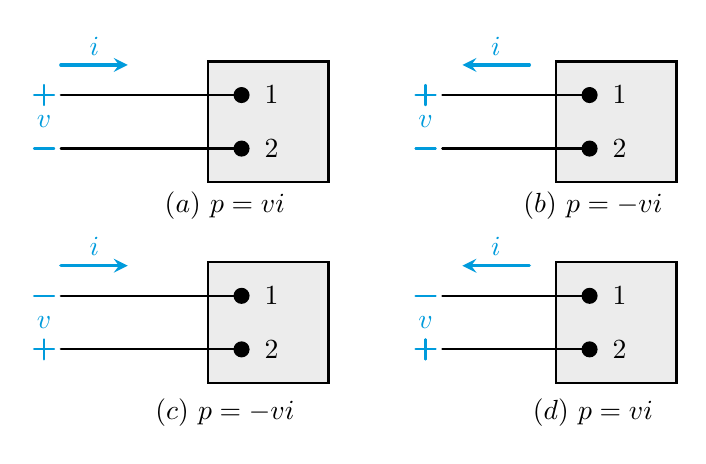
\begin{tikzpicture}[>=stealth, line cap=round, scale=0.85]

    % 一个小电路块的封装:参数为 (是否反极性, 是否反电流方向, 标号)
    % 这里直接展开写,方便你看和改

    % ---------- (a) p = vi ----------
    \begin{scope}[shift={(0,0)}]
      % 灰块和导线
      \fill[gray!15] (1,-0.9) rectangle (2.8,0.9);
      \draw[thick]   (1,-0.9) rectangle (2.8,0.9);
      \draw[thick] (-1.2,0.4) -- (1.5,0.4);
      \draw[thick] (-1.2,-0.4) -- (1.5,-0.4);
      \fill (1.5,0.4) circle (0.12);
      \fill (1.5,-0.4) circle (0.12);
      \node[right] at (1.7,0.4) {$1$};
      \node[right] at (1.7,-0.4) {$2$};

      % 电压极性 + / -
      \draw[elecblue, thick] (-1.6,0.4) -- (-1.3,0.4);
      \draw[elecblue, thick] (-1.45,0.25) -- (-1.45,0.55); % 竖线成 +
      \draw[elecblue, thick] (-1.6,-0.4) -- (-1.3,-0.4);  % -

      % v
      \node[elecblue] at (-1.45,0) {$v$};

      % 电流 i:从左到右
      \draw[elecblue, very thick, ->] (-1.2,0.85) -- (-0.2,0.85);
      \node[above, elecblue] at (-0.7,0.85) {$i$};

      % 标号
      \node at (1.25,-1.25) {$(a)\ p = vi$};
    \end{scope}

    % ---------- (b) p = -vi ----------
    \begin{scope}[shift={(4.5,0)}]
      \fill[gray!15] (1.7,-0.9) rectangle (3.5,0.9);
      \draw[thick]   (1.7,-0.9) rectangle (3.5,0.9);
      \draw[thick] (0,0.4) -- (2.2,0.4);
      \draw[thick] (0,-0.4) -- (2.2,-0.4);
      \fill (2.2,0.4) circle (0.12);
      \fill (2.2,-0.4) circle (0.12);
      \node[right] at (2.4,0.4) {$1$};
      \node[right] at (2.4,-0.4) {$2$};

      % 同样的极性 + / -
      \draw[elecblue, thick] (-0.4,0.4) -- (-0.1,0.4);
      \draw[elecblue, thick] (-0.25,0.25) -- (-0.25,0.55);
      \draw[elecblue, thick] (-0.4,-0.4) -- (-0.1,-0.4);
      \node[elecblue] at (-0.25,0) {$v$};

      % 电流 i:从右到左(反方向)
      \draw[elecblue, very thick, <-] (0.3,0.85) -- (1.3,0.85);
      \node[above, elecblue] at (0.8,0.85) {$i$};

      \node at (2.25,-1.25) {$(b)\ p = -vi$};
    \end{scope}

    % ---------- (c) p = -vi ----------
    \begin{scope}[shift={(0,-3)}]
      \fill[gray!15] (1,-0.9) rectangle (2.8,0.9);
      \draw[thick]   (1,-0.9) rectangle (2.8,0.9);
      \draw[thick] (-1.2,0.4) -- (1.5,0.4);
      \draw[thick] (-1.2,-0.4) -- (1.5,-0.4);
      \fill (1.5,0.4) circle (0.12);
      \fill (1.5,-0.4) circle (0.12);
      \node[right] at (1.7,0.4) {$1$};
      \node[right] at (1.7,-0.4) {$2$};

      % 极性反过来:上端 -
      \draw[elecblue, thick] (-1.6,-0.4) -- (-1.3,-0.4); % 上下对调
      \draw[elecblue, thick] (-1.6,0.4) -- (-1.3,0.4);
      \draw[elecblue, thick] (-1.45,-0.55) -- (-1.45,-0.25); % + 在下端
      \node[elecblue] at (-1.45,0) {$v$};

      % 电流 i:从左到右
      \draw[elecblue, very thick, ->] (-1.2,0.85) -- (-0.2,0.85);
      \node[above, elecblue] at (-0.7,0.85) {$i$};

      \node at (1.25,-1.35) {$(c)\ p = -vi$};
    \end{scope}

    % ---------- (d) p = vi ----------
    \begin{scope}[shift={(4.5,-3)}]
      \fill[gray!15] (1.7,-0.9) rectangle (3.5,0.9);
      \draw[thick]   (1.7,-0.9) rectangle (3.5,0.9);
      \draw[thick] (0,0.4) -- (2.2,0.4);
      \draw[thick] (0,-0.4) -- (2.2,-0.4);
      \fill (2.2,0.4) circle (0.12);
      \fill (2.2,-0.4) circle (0.12);
      \node[right] at (2.4,0.4) {$1$};
      \node[right] at (2.4,-0.4) {$2$};

      % 极性反过来
      \draw[elecblue, thick] (-0.4,-0.4) -- (-0.1,-0.4);
      \draw[elecblue, thick] (-0.4,0.4) -- (-0.1,0.4);
      \draw[elecblue, thick] (-0.25,-0.55) -- (-0.25,-0.25);
      \node[elecblue] at (-0.25,0) {$v$};

      % 电流 i:从右到左
      \draw[elecblue, very thick, <-] (0.3,0.85) -- (1.3,0.85);
      \node[above, elecblue] at (0.8,0.85) {$i$};

      \node at (2.25,-1.35) {$(d)\ p = vi$};
    \end{scope}

  \end{tikzpicture}

 PSC 下:
\begin{itemize}
  \item $p=vi>0$:电荷沿电压\emph{下降}方向流动,\textbf{失去}电能,元件吸收功率(如电阻、负载)。
  \item $p=vi<0$:电荷沿电压\emph{上升}方向流动,\textbf{获得}电能,元件对外供能(如理想源)。
\end{itemize}

若电流参考方向与电压极性相反,需写成 $p=-vi$,物理解释保持不变。

\subsection{电路的“功率平衡”思想}
\noindent 对于只含\textbf{线性、集中参数元件}的电路:
\paragraph*{}在任意时刻,\textbf{所有元件功率代数和应为 0}:
  \[
    \sum\limits_{\text{all elements}} p_k(t) = 0.
  \]
\begin{itemize}
\item 即“源件发出的总功率”=“负载吸收的总功率”。
\end{itemize}
\end{document}